\begin{itemize}
\item Eine Fotozelle wird mit UV-Licht bestrahlt, dadurch werden Elektronen $e^-$ aus der Kathode ausgelöst (Natrium). Es wird eine Gegenspannung $U_{max}$ angelegt und so lange erhöht, bis kein Strom I mehr gemessen wird.

Die herausgeschlagenen $e^-$ besitzen eine kinetische Energie $E_{kin}$. Durch die Gegenspannung müssen sie gegen ein elektrisches Feld "ankämpfen". Wenn kein Strom I mehr gemessen wird ist die elektrische Energie $E_{el} = U \cdot e$ gleich der kinetischen Energie $E_{kin} = \dfrac{1}{2} m v^2$.
\item Im nächsten Schritt wird die maximale kinetische Energie (uns interessieren nur die schnellsten Elektronen) der Photonenenergie abzüglich der minimalen Austrittsarbeit, die notwendig ist um ein Elektron überhaupt aus der Platt zu lösen, gleich gesetzt.

$E_{kin,max} = E_{phot} - W_A$ ; Der Unterschied zwischen Arbeit und Energie ist philosophischer Natur, d.h. Energie und Arbeit haben die selben Einheiten.
\item Daraus folgt die Einstein'sche Gleichung: \\ 
$E_{kin,max} = h \cdot f - W_A$ \tabto{0.5\textwidth} ; $E_{phot} = h \cdot f$ \\
$E_{el} = E_{kin,max}$ \\
$e \cdot U = h \cdot f - W_A$ \tabto{0.5\textwidth} ; $E_{el} = e \cdot U$
\item Das Plack'sches Wirkungsquantum $h$ ist konstant: $h = 6,626\cdot10^{-34} Js$ [$\frac{kg \ m^2}{s^2} \cdot s$]
\item Die Grenzfrequenz $f_{gr}$ ist die Frequenz ab der Elektronen ausgelöst werden, sie ist Material abhängig.

$W_A = h \cdot f_{gr} \rightarrow f_{gr} = \frac{W_A}{h}$
\end{itemize}

\begin{figure}[h!]
\centering 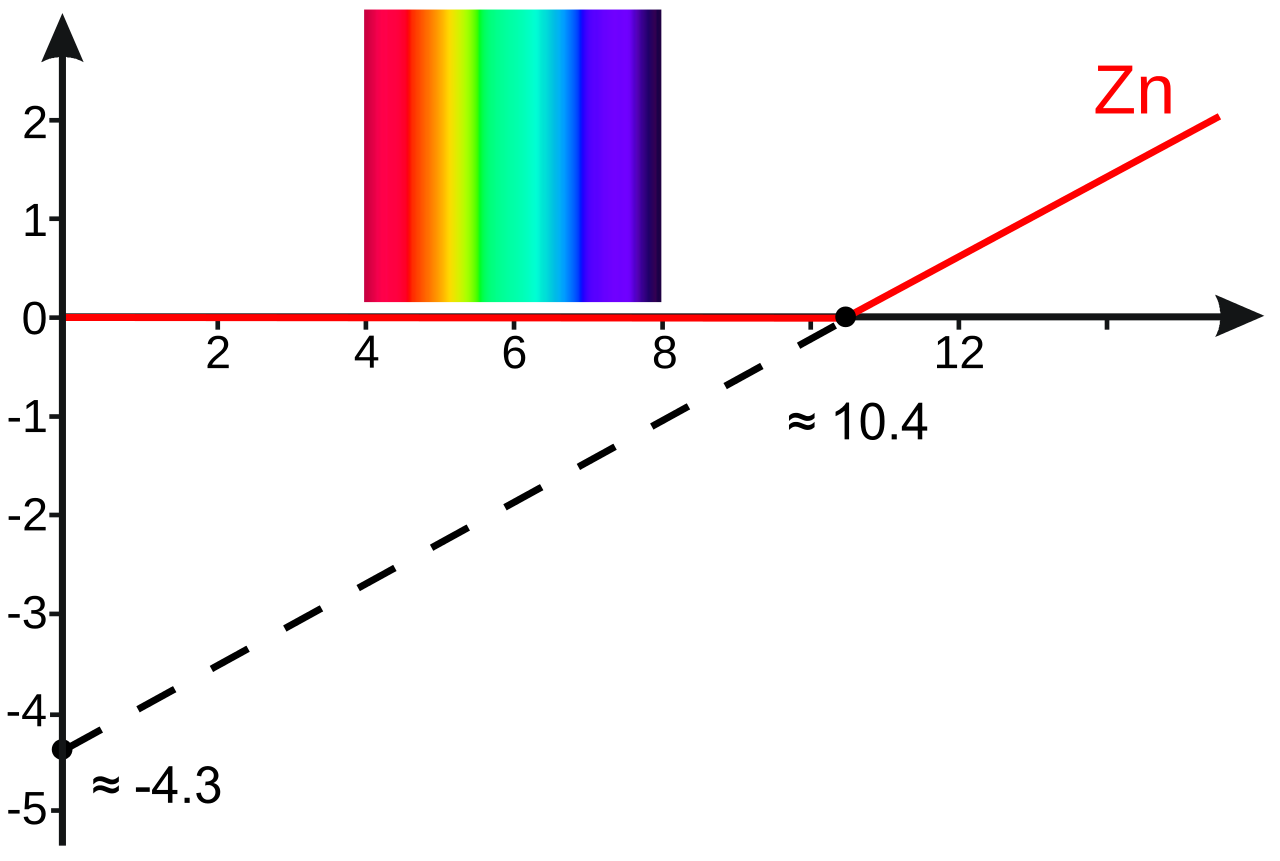
\includegraphics[width=0.8\textwidth]{Photoelectric_effect_diagram_no_label}
\caption{Abbildung von: \url{https://upload.wikimedia.org/wikipedia/commons/thumb/5/54/Photoelectric\_effect\_diagram\_no\_label.svg/1280px-Photoelectric\_effect\_diagram\_no\_label.svg.png}}
\end{figure}